\section{ATMS NPP channel SRF comparisons}
%==============================================
\label{app:srf}
This appendix plots the various NPP ATMS microwave spectral response functions (SRFs) used in this study. The "boxcar" data is derived from the data shown in table \ref{tab:atms_fo_sb_and_df}, the "Table 12" data is an edited form of the data from table 12 in reference \cite{ATMS_PFM_CalLog}, and the SDL \cite{ATMS_SRF_SDL} and NGAS \cite{ATMS_SRF_NGAS} data are digitisations of various measured ATMS channel response plots shown in reference \cite{ATMS_PFM_CalLog}.

\newpage

% Note: the "[H]" placement option is allowed due to the use of the float package
%       in the preamble. I did this to avoid the
%        ! LaTeX Error: Too many unprocessed floats.
%       error due to the large number of figures.

\begin{figure}[H]
  \centering
  \begin{tabular}{c}
    \includegraphics[scale=1]{graphics/srf/atms_npp.ch1.srf.eps} \\
    % the hand-crafted legend
    \setlength{\unitlength}{1cm}
    \begin{picture}(2.0,0.0)(0.0,-2.0)
      \thicklines
      \color{green}
      \put(0.0,0.7 ){\line(1,0){1}}
      \put(1.1,0.55){\sffamily SDL}
      \color{red}
      \put(0.0,1.2 ){\line(1,0){1}}
      \put(1.1,1.05){\sffamily Table 12}
      \color{black}
      \put(0.0,1.7 ){\line(1,0){1}}
      \put(1.1,1.55){\sffamily Boxcar}
    \end{picture} \\\\
    \includegraphics[bb=249 194 1431 1035,scale=0.3]{graphics/log_book/ch1.eps}
  \end{tabular}
  \caption{NPP ATMS channel 1 response. \textbf{(Top)} Boxcar and digitised data. \textbf{(Bottom)} Nominal filter response from ATMS Calibration Data Book\cite{ATMS_PFM_CalLog}.}
  \label{fig:atms_npp.ch1.srf}
\end{figure}

\begin{figure}[H]
  \centering
  \includegraphics[scale=1]{graphics/srf/atms_npp.ch2.srf.eps}
  % the hand-crafted legend
  \setlength{\unitlength}{1cm}
  \begin{picture}(2.0,0.0)(0.0,-2.0)
    \thicklines
    \color{red}
    \put(0.0,1.2 ){\line(1,0){1}}
    \put(1.1,1.05){\sffamily Table 12}
    \color{black}
    \put(0.0,1.7 ){\line(1,0){1}}
    \put(1.1,1.55){\sffamily Boxcar}
  \end{picture}
  \caption{NPP ATMS channel 2 response.}
  \label{fig:atms_npp.ch2.srf}
\end{figure}

\begin{figure}[H]
  \centering
  \includegraphics[scale=1]{graphics/srf/atms_npp.ch3.srf.eps}
  % the hand-crafted legend
  \setlength{\unitlength}{1cm}
  \begin{picture}(2.0,0.0)(0.0,-2.0)
    \thicklines
    \color{red}
    \put(0.0,1.2 ){\line(1,0){1}}
    \put(1.1,1.05){\sffamily Table 12}
    \color{black}
    \put(0.0,1.7 ){\line(1,0){1}}
    \put(1.1,1.55){\sffamily Boxcar}
  \end{picture}
  \caption{NPP ATMS channel 3 response.}
  \label{fig:atms_npp.ch3.srf}
\end{figure}

\begin{figure}[H]
  \centering
  \begin{tabular}{c}
    \includegraphics[scale=1]{graphics/srf/atms_npp.ch4.srf.eps} \\
    % the hand-crafted legend
    \setlength{\unitlength}{1cm}
    \begin{picture}(2.0,0.0)(0.0,-2.0)
      \thicklines
      \color{blue}
      \put(0.0,0.7 ){\line(1,0){1}}
      \put(1.1,0.55){\sffamily NGAS}
      \color{red}
      \put(0.0,1.2 ){\line(1,0){1}}
      \put(1.1,1.05){\sffamily Table 12}
      \color{black}
      \put(0.0,1.7 ){\line(1,0){1}}
      \put(1.1,1.55){\sffamily Boxcar}
    \end{picture} \\\\
    \includegraphics[bb=249 194 1431 1035,scale=0.3]{graphics/log_book/ch4.eps}
  \end{tabular}
  \caption{NPP ATMS channel 4 response. \textbf{(Top)} Boxcar and digitised data. \textbf{(Bottom)} Nominal filter response from ATMS Calibration Data Book\cite{ATMS_PFM_CalLog}.}
  \label{fig:atms_npp.ch4.srf}
\end{figure}

\begin{figure}[H]
  \centering
  \begin{tabular}{c}
    \includegraphics[scale=1]{graphics/srf/atms_npp.ch5.srf.eps} \\
    % the hand-crafted legend
    \setlength{\unitlength}{1cm}
    \begin{picture}(2.0,0.0)(0.0,-2.0)
      \thicklines
      \color{blue}
      \put(0.0,0.7 ){\line(1,0){1}}
      \put(1.1,0.55){\sffamily NGAS}
      \color{red}
      \put(0.0,1.2 ){\line(1,0){1}}
      \put(1.1,1.05){\sffamily Table 12}
      \color{black}
      \put(0.0,1.7 ){\line(1,0){1}}
      \put(1.1,1.55){\sffamily Boxcar}
    \end{picture} \\\\
    \includegraphics[bb=249 194 1431 1035,scale=0.3]{graphics/log_book/ch5.eps}
  \end{tabular}
  \caption{NPP ATMS channel 5 response. \textbf{(Top)} Boxcar and digitised data. \textbf{(Bottom)} Nominal filter response from ATMS Calibration Data Book\cite{ATMS_PFM_CalLog}.}
  \label{fig:atms_npp.ch5.srf}
\end{figure}

\begin{figure}[H]
  \centering
  \includegraphics[scale=1]{graphics/srf/atms_npp.ch6.srf.eps}
  % the hand-crafted legend
  \setlength{\unitlength}{1cm}
  \begin{picture}(2.0,0.0)(3.0,-2.0)
    \thicklines
    \color{red}
    \put(0.0,1.2 ){\line(1,0){1}}
    \put(1.1,1.05){\sffamily Table 12}
    \color{black}
    \put(0.0,1.7 ){\line(1,0){1}}
    \put(1.1,1.55){\sffamily Boxcar}
  \end{picture}
  \caption{NPP ATMS channel 6 response.}
  \label{fig:atms_npp.ch6.srf}
\end{figure}

\begin{figure}[H]
  \centering
  \includegraphics[scale=1]{graphics/srf/atms_npp.ch7.srf.eps}
  % the hand-crafted legend
  \setlength{\unitlength}{1cm}
  \begin{picture}(2.0,0.0)(0.0,-2.0)
    \thicklines
    \color{red}
    \put(0.0,1.2 ){\line(1,0){1}}
    \put(1.1,1.05){\sffamily Table 12}
    \color{black}
    \put(0.0,1.7 ){\line(1,0){1}}
    \put(1.1,1.55){\sffamily Boxcar}
  \end{picture}
  \caption{NPP ATMS channel 7 response.}
  \label{fig:atms_npp.ch7.srf}
\end{figure}

\begin{figure}[H]
  \centering
  \includegraphics[scale=1]{graphics/srf/atms_npp.ch8.srf.eps}
  % the hand-crafted legend
  \setlength{\unitlength}{1cm}
  \begin{picture}(2.0,0.0)(0.0,-2.0)
    \thicklines
    \color{red}
    \put(0.0,1.2 ){\line(1,0){1}}
    \put(1.1,1.05){\sffamily Table 12}
    \color{black}
    \put(0.0,1.7 ){\line(1,0){1}}
    \put(1.1,1.55){\sffamily Boxcar}
  \end{picture}
  \caption{NPP ATMS channel 8 response.}
  \label{fig:atms_npp.ch8.srf}
\end{figure}

\begin{figure}[H]
  \centering
  \begin{tabular}{c}
    \includegraphics[scale=1]{graphics/srf/atms_npp.ch9.srf.eps} \\
    % the hand-crafted legend
    \setlength{\unitlength}{1cm}
    \begin{picture}(2.0,0.0)(0.0,-2.0)
      \thicklines
      \color{blue}
      \put(0.0,0.7 ){\line(1,0){1}}
      \put(1.1,0.55){\sffamily NGAS}
      \color{red}
      \put(0.0,1.2 ){\line(1,0){1}}
      \put(1.1,1.05){\sffamily Table 12}
      \color{black}
      \put(0.0,1.7 ){\line(1,0){1}}
      \put(1.1,1.55){\sffamily Boxcar}
    \end{picture} \\\\
    \includegraphics[bb=249 194 1431 1035,scale=0.3]{graphics/log_book/ch9.eps}
  \end{tabular}
  \caption{NPP ATMS channel 9 response. \textbf{(Top)} Boxcar and digitised data. \textbf{(Bottom)} Nominal filter response from ATMS Calibration Data Book\cite{ATMS_PFM_CalLog}.}
  \label{fig:atms_npp.ch9.srf}
\end{figure}

\begin{figure}[H]
  \centering
  \includegraphics[scale=1]{graphics/srf/atms_npp.ch10.srf.eps}
  % the hand-crafted legend
  \setlength{\unitlength}{1cm}
  \begin{picture}(2.0,0.0)(0.0,-2.0)
    \thicklines
    \color{red}
    \put(0.0,1.2 ){\line(1,0){1}}
    \put(1.1,1.05){\sffamily Table 12}
    \color{black}
    \put(0.0,1.7 ){\line(1,0){1}}
    \put(1.1,1.55){\sffamily Boxcar}
  \end{picture}
  \caption{NPP ATMS channel 10 response.}
  \label{fig:atms_npp.ch10.srf}
\end{figure}

\begin{figure}[H]
  \centering
  \includegraphics[scale=1]{graphics/srf/atms_npp.ch11.srf.eps}
  % the hand-crafted legend
  \setlength{\unitlength}{1cm}
  \begin{picture}(2.0,0.0)(3.5,-2.0)
    \thicklines
    \color{red}
    \put(0.0,1.2 ){\line(1,0){1}}
    \put(1.1,1.05){\sffamily Table 12}
    \color{black}
    \put(0.0,1.7 ){\line(1,0){1}}
    \put(1.1,1.55){\sffamily Boxcar}
  \end{picture}
  \caption{NPP ATMS channel 11 response.}
  \label{fig:atms_npp.ch11.srf}
\end{figure}

\begin{figure}[H]
  \centering
  \begin{tabular}{c c}
    \multicolumn{2}{c}{\includegraphics[scale=1]{graphics/srf/atms_npp.ch12.srf.eps}}\\
    % the hand-crafted legend
    \multicolumn{2}{c}{
      \setlength{\unitlength}{1cm}
      \begin{picture}(2.0,0.0)(1.7,-1.2)
        \thicklines
        \color{green}
        \put(0.0,0.7 ){\line(1,0){1}}
        \put(1.1,0.55){\sffamily SDL}
        \color{red}
        \put(0.0,1.2 ){\line(1,0){1}}
        \put(1.1,1.05){\sffamily Table 12}
        \color{black}
        \put(0.0,1.7 ){\line(1,0){1}}
        \put(1.1,1.55){\sffamily Boxcar}
      \end{picture}} \\\\
    \includegraphics[bb=249 194 1431 1035,scale=0.2]{graphics/log_book/ch12_lowf.eps} & 
    \includegraphics[bb=249 194 1431 1035,scale=0.2]{graphics/log_book/ch12_hif.eps}
  \end{tabular}
  \caption{NPP ATMS channel 12 response. \textbf{(Top)} Boxcar and digitised data. \textbf{(Bottom)} Nominal filter (low and high IF) response from ATMS Calibration Data Book\cite{ATMS_PFM_CalLog}. The low IF (left) reponsse corresponds to band \#3 and the high IF (right) response to band \#4.}
  \label{fig:atms_npp.ch12.srf}
\end{figure}

\begin{figure}[H]
  \centering
  \begin{tabular}{c c}
    \multicolumn{2}{c}{\includegraphics[scale=1]{graphics/srf/atms_npp.ch13.srf.eps}}\\
    % the hand-crafted legend
    \multicolumn{2}{c}{
      \setlength{\unitlength}{1cm}
      \begin{picture}(2.0,0.0)(1.7,-1.6)
        \thicklines
        \color{blue}
        \put(0.0,0.2 ){\line(1,0){1}}
        \put(1.1,0.05){\sffamily NGAS}
        \color{green}
        \put(0.0,0.7 ){\line(1,0){1}}
        \put(1.1,0.55){\sffamily SDL}
        \color{red}
        \put(0.0,1.2 ){\line(1,0){1}}
        \put(1.1,1.05){\sffamily Table 12}
        \color{black}
        \put(0.0,1.7 ){\line(1,0){1}}
        \put(1.1,1.55){\sffamily Boxcar}
      \end{picture}} \\\\
    \includegraphics[bb=249 194 1431 1035,scale=0.2]{graphics/log_book/ch13_lowf.eps} & 
    \includegraphics[bb=249 194 1431 1035,scale=0.2]{graphics/log_book/ch13_hif.eps}
  \end{tabular}
  \caption{NPP ATMS channel 13 response. \textbf{(Top)} Boxcar and digitised data. \textbf{(Bottom)} Nominal filter (low and high IF) response from ATMS Calibration Data Book\cite{ATMS_PFM_CalLog}. The low IF (left) reponsse corresponds to band \#3 and the high IF (right) response to band \#4.}
  \label{fig:atms_npp.ch13.srf}
\end{figure}

\begin{figure}[H]
  \centering
  \begin{tabular}{c c}
    \multicolumn{2}{c}{\includegraphics[scale=1]{graphics/srf/atms_npp.ch14.srf.eps}}\\
    % the hand-crafted legend
    \multicolumn{2}{c}{
      \setlength{\unitlength}{1cm}
      \begin{picture}(2.0,0.0)(1.7,-1.6)
        \thicklines
        \color{blue}
        \put(0.0,0.2 ){\line(1,0){1}}
        \put(1.1,0.05){\sffamily NGAS}
        \color{green}
        \put(0.0,0.7 ){\line(1,0){1}}
        \put(1.1,0.55){\sffamily SDL}
        \color{red}
        \put(0.0,1.2 ){\line(1,0){1}}
        \put(1.1,1.05){\sffamily Table 12}
        \color{black}
        \put(0.0,1.7 ){\line(1,0){1}}
        \put(1.1,1.55){\sffamily Boxcar}
      \end{picture}} \\\\
    \includegraphics[bb=249 194 1431 1035,scale=0.2]{graphics/log_book/ch14_lowf.eps} & 
    \includegraphics[bb=249 194 1431 1035,scale=0.2]{graphics/log_book/ch14_hif.eps}
  \end{tabular}
  \caption{NPP ATMS channel 14 response. \textbf{(Top)} Boxcar and digitised data. \textbf{(Bottom)} Nominal filter (low and high IF) response from ATMS Calibration Data Book\cite{ATMS_PFM_CalLog}. The low IF (left) reponsse corresponds to band \#3 and the high IF (right) response to band \#4.}
  \label{fig:atms_npp.ch14.srf}
\end{figure}

\begin{figure}[H]
  \centering
  \begin{tabular}{c c}
    \multicolumn{2}{c}{\includegraphics[scale=1]{graphics/srf/atms_npp.ch15.srf.eps}}\\
    % the hand-crafted legend
    \multicolumn{2}{c}{
      \setlength{\unitlength}{1cm}
      \begin{picture}(2.0,0.0)(1.7,-1.2)
        \thicklines
        \color{green}
        \put(0.0,0.7 ){\line(1,0){1}}
        \put(1.1,0.55){\sffamily SDL}
        \color{red}
        \put(0.0,1.2 ){\line(1,0){1}}
        \put(1.1,1.05){\sffamily Table 12}
        \color{black}
        \put(0.0,1.7 ){\line(1,0){1}}
        \put(1.1,1.55){\sffamily Boxcar}
      \end{picture}} \\\\
    \includegraphics[bb=249 194 1431 1035,scale=0.2]{graphics/log_book/ch15_lowf.eps} & 
    \includegraphics[bb=249 194 1431 1035,scale=0.2]{graphics/log_book/ch15_hif.eps}
  \end{tabular}
  \caption{NPP ATMS channel 15 response. \textbf{(Top)} Boxcar and digitised data. \textbf{(Bottom)} Nominal filter (low and high IF) response from ATMS Calibration Data Book\cite{ATMS_PFM_CalLog}. The low IF (left) reponsse corresponds to band \#3 and the high IF (right) response to band \#4.}
  \label{fig:atms_npp.ch15.srf}
\end{figure}

\begin{figure}[H]
  \centering
  \includegraphics[scale=1]{graphics/srf/atms_npp.ch16.srf.eps}
  % the hand-crafted legend
  \setlength{\unitlength}{1cm}
  \begin{picture}(2.0,0.0)(0.0,-2.0)
    \thicklines
    \color{red}
    \put(0.0,1.2 ){\line(1,0){1}}
    \put(1.1,1.05){\sffamily Table 12}
    \color{black}
    \put(0.0,1.7 ){\line(1,0){1}}
    \put(1.1,1.55){\sffamily Boxcar}
  \end{picture}
  \caption{NPP ATMS channel 16 response.}
  \label{fig:atms_npp.ch16.srf}
\end{figure}

\begin{figure}[H]
  \centering
  \includegraphics[scale=1]{graphics/srf/atms_npp.ch17.srf.eps}
  % the hand-crafted legend
  \setlength{\unitlength}{1cm}
  \begin{picture}(2.0,0.0)(0.0,-2.0)
    \thicklines
    \color{red}
    \put(0.0,1.2 ){\line(1,0){1}}
    \put(1.1,1.05){\sffamily Table 12}
    \color{black}
    \put(0.0,1.7 ){\line(1,0){1}}
    \put(1.1,1.55){\sffamily Boxcar}
  \end{picture}
  \caption{NPP ATMS channel 17 response.}
  \label{fig:atms_npp.ch17.srf}
\end{figure}

\begin{figure}[H]
  \centering
  \includegraphics[scale=1]{graphics/srf/atms_npp.ch18.srf.eps}
  % the hand-crafted legend
  \setlength{\unitlength}{1cm}
  \begin{picture}(2.0,0.0)(3.5,-2.0)
    \thicklines
    \color{red}
    \put(0.0,1.2 ){\line(1,0){1}}
    \put(1.1,1.05){\sffamily Table 12}
    \color{black}
    \put(0.0,1.7 ){\line(1,0){1}}
    \put(1.1,1.55){\sffamily Boxcar}
  \end{picture}
  \caption{NPP ATMS channel 18 response.}
  \label{fig:atms_npp.ch18.srf}
\end{figure}

\begin{figure}[H]
  \centering
  \includegraphics[scale=1]{graphics/srf/atms_npp.ch19.srf.eps}
  % the hand-crafted legend
  \setlength{\unitlength}{1cm}
  \begin{picture}(2.0,0.0)(5.0,-3.0)
    \thicklines
    \color{red}
    \put(0.0,1.2 ){\line(1,0){1}}
    \put(1.1,1.05){\sffamily Table 12}
    \color{black}
    \put(0.0,1.7 ){\line(1,0){1}}
    \put(1.1,1.55){\sffamily Boxcar}
  \end{picture}
  \caption{NPP ATMS channel 19 response.}
  \label{fig:atms_npp.ch19.srf}
\end{figure}

\begin{figure}[H]
  \centering
  \includegraphics[scale=1]{graphics/srf/atms_npp.ch20.srf.eps}
  % the hand-crafted legend
  \setlength{\unitlength}{1cm}
  \begin{picture}(2.0,0.0)(3.5,-2.0)
    \thicklines
    \color{red}
    \put(0.0,1.2 ){\line(1,0){1}}
    \put(1.1,1.05){\sffamily Table 12}
    \color{black}
    \put(0.0,1.7 ){\line(1,0){1}}
    \put(1.1,1.55){\sffamily Boxcar}
  \end{picture}
  \caption{NPP ATMS channel 20 response.}
  \label{fig:atms_npp.ch20.srf}
\end{figure}

\begin{figure}[H]
  \centering
  \includegraphics[scale=1]{graphics/srf/atms_npp.ch21.srf.eps}
  % the hand-crafted legend
  \setlength{\unitlength}{1cm}
  \begin{picture}(2.0,0.0)(3.5,-2.0)
    \thicklines
    \color{red}
    \put(0.0,1.2 ){\line(1,0){1}}
    \put(1.1,1.05){\sffamily Table 12}
    \color{black}
    \put(0.0,1.7 ){\line(1,0){1}}
    \put(1.1,1.55){\sffamily Boxcar}
  \end{picture}
  \caption{NPP ATMS channel 21 response.}
  \label{fig:atms_npp.ch21.srf}
\end{figure}

\begin{figure}[H]
  \centering
  \includegraphics[scale=1]{graphics/srf/atms_npp.ch22.srf.eps}
  % the hand-crafted legend
  \setlength{\unitlength}{1cm}
  \begin{picture}(2.0,0.0)(3.5,-2.0)
    \thicklines
    \color{red}
    \put(0.0,1.2 ){\line(1,0){1}}
    \put(1.1,1.05){\sffamily Table 12}
    \color{black}
    \put(0.0,1.7 ){\line(1,0){1}}
    \put(1.1,1.55){\sffamily Boxcar}
  \end{picture}
  \caption{NPP ATMS channel 22 response.}
  \label{fig:atms_npp.ch22.srf}
\end{figure}
